% This is "sig-alternate.tex" V2.1 April 2013
% This file should be compiled with V2.5 of "sig-alternate.cls" May 2012
%
% This example file demonstrates the use of the 'sig-alternate.cls'
% V2.5 LaTeX2e document class file. It is for those submitting
% articles to ACM Conference Proceedings WHO DO NOT WISH TO
% STRICTLY ADHERE TO THE SIGS (PUBS-BOARD-ENDORSED) STYLE.
% The 'sig-alternate.cls' file will produce a similar-looking,
% albeit, 'tighter' paper resulting in, invariably, fewer pages.
%
% ----------------------------------------------------------------------------------------------------------------
% This .tex file (and associated .cls V2.5) produces:
%       1) The Permission Statement
%       2) The Conference (location) Info information
%       3) The Copyright Line with ACM data
%       4) NO page numbers
%
% as against the acm_proc_article-sp.cls file which
% DOES NOT produce 1) thru' 3) above.
%
% Using 'sig-alternate.cls' you have control, however, from within
% the source .tex file, over both the CopyrightYear
% (defaulted to 200X) and the ACM Copyright Data
% (defaulted to X-XXXXX-XX-X/XX/XX).
% e.g.
% \CopyrightYear{2007} will cause 2007 to appear in the copyright line.
% \crdata{0-12345-67-8/90/12} will cause 0-12345-67-8/90/12 to appear in the copyright line.
%
% ---------------------------------------------------------------------------------------------------------------
% This .tex source is an example which *does* use
% the .bib file (from which the .bbl file % is produced).
% REMEMBER HOWEVER: After having produced the .bbl file,
% and prior to final submission, you *NEED* to 'insert'
% your .bbl file into your source .tex file so as to provide
% ONE 'self-contained' source file.
%
% ================= IF YOU HAVE QUESTIONS =======================
% Questions regarding the SIGS styles, SIGS policies and
% procedures, Conferences etc. should be sent to
% Adrienne Griscti (griscti@acm.org)
%
% Technical questions _only_ to
% Gerald Murray (murray@hq.acm.org)
% ===============================================================
%
% For tracking purposes - this is V2.0 - May 2012

%\documentclass{sig-alternate-05-2015}

\documentclass{sig-alternate-05-2015}
\usepackage{textcomp}
\usepackage{biblatex}
\addbibresource{BibDRL.bib}
\addbibresource{BibMBS.bib}
\usepackage{acmcopyright}
\begin{document}

% Copyright
\setcopyright{acmcopyright}
%\setcopyright{acmlicensed}
%\setcopyright{rightsretained}
%\setcopyright{usgov}
%\setcopyright{usgovmixed}
%\setcopyright{cagov}
%\setcopyright{cagovmixed}


% DOI
\doi{10.1145/3365265.3365274}

% ISBN
\isbn{978-1-4503-7288-6/19/10}

%Conference
\conferenceinfo{ICACR 2019,}{\emph{October 11--13, 2019 Prague, Czech Republic}}

\acmPrice{\$15.00}

%
% --- Author Metadata here ---

\CopyrightYear{2019} % Allows default copyright year (20XX) to be over-ridden - IF NEED BE.
%\crdata{0-12345-67-8/90/01}  % Allows default copyright data (0-89791-88-6/97/05) to be over-ridden - IF NEED BE.
% --- End of Author Metadata ---

\title{A Modular Simulation Platform for Training Robots via Deep Reinforcement Learning and Multibody Dynamics}

%\subtitle{[Extended Abstract]
%\titlenote{A full version of this paper is available as
%\textit{Author's Guide to Preparing ACM SIG Proceedings Using
%\LaTeX$2_\epsilon$\ and BibTeX} at
%\texttt{www.acm.org/eaddress.htm}}}

%
% You need the command \numberofauthors to handle the 'placement
% and alignment' of the authors beneath the title.
%
% For aesthetic reasons, we recommend 'three authors at a time'
% i.e. three 'name/affiliation blocks' be placed beneath the title.
%
% NOTE: You are NOT restricted in how many 'rows' of
% "name/affiliations" may appear. We just ask that you restrict
% the number of 'columns' to three.
%
% Because of the available 'opening page real-estate'
% we ask you to refrain from putting more than six authors
% (two rows with three columns) beneath the article title.
% More than six makes the first-page appear very cluttered indeed.
%
% Use the \alignauthor commands to handle the names
% and affiliations for an 'aesthetic maximum' of six authors.
% Add names, affiliations, addresses for
% the seventh etc. author(s) as the argument for the
% \additionalauthors command.
% These 'additional authors' will be output/set for you
% without further effort on your part as the last section in
% the body of your article BEFORE References or any Appendices.

\numberofauthors{6} %  in this sample file, there are a *total*
% of EIGHT authors. SIX appear on the 'first-page' (for formatting
% reasons) and the remaining two appear in the \additionalauthors section.
%
\author{
% You can go ahead and credit any number of authors here,
% e.g. one 'row of three' or two rows (consisting of one row of three
% and a second row of one, two or three).
%
% The command \alignauthor (no curly braces needed) should
% precede each author name, affiliation/snail-mail address and
% e-mail address. Additionally, tag each line of
% affiliation/address with \affaddr, and tag the
% e-mail address with \email.
%
% 1st. author
\alignauthor
Simone Benatti\titlenote{Corresponding Author}\\
       \affaddr{University of Parma Dpt. of Engineering and Architecture}\\
       \affaddr{Parco Area delle Scienze, 181/A}\\
       \affaddr{Parma, Italy}\\
       \email{simone.benatti@\linebreak[0]studenti.unipr.it}
% 2nd. author
\alignauthor
Alessandro Tasora\\
       \affaddr{University of Parma Dpt. of Engineering and Architecture}\\
       \affaddr{Parco Area delle Scienze, 181/A}\\
       \affaddr{Parma, Italy}\\
       \email{alessandro.tasora@unipr.it}
% 3rd. author
\alignauthor 
Dario Fusai\\
       \affaddr{University of Parma Dpt. of Engineering and Architecture}\\
       \affaddr{Parco Area delle Scienze, 181/A}\\
       \affaddr{Parma, Italy}\\
       \email{dario.fusai@unipr.it}
\and  % use '\and' if you need 'another row' of author names
% 4th. author
Dario Mangoni\\
       \affaddr{University of Parma Dpt. of Engineering and Architecture}\\
       \affaddr{Parco Area delle Scienze, 181/A}\\
       \affaddr{Parma, Italy}\\
       \email{dario.mangoni@unipr.it}
}
% There's nothing stopping you putting the seventh, eighth, etc.
% author on the opening page (as the 'third row') but we ask,
% for aesthetic reasons that you place these 'additional authors'
% in the \additional authors block, viz.
\additionalauthors{Additional authors: John Smith (The Th{\o}rv{\"a}ld Group,
email: {\texttt{jsmith@affiliation.org}}) and Julius P.~Kumquat
(The Kumquat Consortium, email: {\texttt{jpkumquat@consortium.net}}).}
\date{30 July 1999}
% Just remember to make sure that the TOTAL number of authors
% is the number that will appear on the first page PLUS the
% number that will appear in the \additionalauthors section.

\maketitle
\begin{abstract}
In this work we focus on the role of Multibody Simulation in creating Reinforcement Learning virtual environments for robotic manipulation, showing a versatile, efficient and open source toolchain to create directly from CAD models.
Using the Chrono::Solidworks plugin we are able to create robotic environments in the 3D CAD software Solidworks\textregistered and later convert them into PyChrono models (PyChrono is an open source Python module for multibody simulation).
In addition, we demonstrate how collision detection can be made more efficient by introducing a limited number of contact primitives instead of performing collision detection and evaluation on complex 3D meshes, still reaching a policy able to avoid unwanted collisions.
We tested this approach on a 6DOF robot Comau Racer3: the robot, together with a 2 fingers gripper (Hand-E by Robotiq) was modelled using Solidworks\textregistered, imported as a PyChrono model and then a NN was trained in simulation to control its motor torques to reach a target position.
To demonstrate the versatility of this toolchain we also repeated the same procedure to model and then train the ABB IRB 120 robotic arm.

\end{abstract}


%
% The code below should be generated by the tool at
% http://dl.acm.org/ccs.cfm
% Please copy and paste the code instead of the example below. 
%
\begin{CCSXML}
<ccs2012>
<concept>
<concept_id>10003752.10010070.10010071.10010261</concept_id>
<concept_desc>Theory of computation~Reinforcement learning</concept_desc>
<concept_significance>500</concept_significance>
</concept>
<concept>
<concept_id>10010147.10010371.10010352.10010379</concept_id>
<concept_desc>Computing methodologies~Physical simulation</concept_desc>
<concept_significance>500</concept_significance>
</concept>
<concept>
<concept_id>10010147.10010257.10010293.10010294</concept_id>
<concept_desc>Computing methodologies~Neural networks</concept_desc>
<concept_significance>300</concept_significance>
</concept>
<concept>
<concept_id>10010520.10010553.10010554.10010556</concept_id>
<concept_desc>Computer systems organization~Robotic control</concept_desc>
<concept_significance>100</concept_significance>
</concept>
</ccs2012>
\end{CCSXML}

\ccsdesc[500]{Theory of computation~Reinforcement learning}
\ccsdesc[500]{Computing methodologies~Physical simulation}
\ccsdesc[300]{Computing methodologies~Neural networks}
\ccsdesc[100]{Computer systems organization~Robotic control}
%
% End generated code
%

%
%  Use this command to print the description
%
\printccsdesc

% We no longer use \terms command
%\terms{Theory}

\keywords{Physical Simulation; Multibody Simulation; Reinforcement Learning; Deep Learning; Neural Networks; Robotics; Control}

\section{Introduction}
Since its introduction \cite{Mnih13}, Deep Reinforcement Learning has been applied successfully to a wide range of applications in robotic grasping \cite{Levine2016} \cite{LevineFDA15} and dexterous manipulation \cite{openai2018HandManipulation}.

This being said, the role of simulation so far has been primarily aimed to benchmarking of DRL algorithms in continuous state-action tasks. In this context, model definition through xml files using URDF syntax is totally appropriate, favoring the model sharing, however, this approach lacks of versatility.
Since the next years will probably see an increasing diffusion of industrial applications of DRL for robotic control, there will be a major interest in the ability of creating tailored and efficient training environments. 
For this reason we developed and tested a toolchain which allows to create Multibody Simulation models from CAD and use them to train NN. 

In addition , we want to demonstrate that in most cases there is no need to perform collision detection and evaluate contact forces on complex triangular meshes, and a limited number of primitive contact shapes placed in critical points is sufficient for the agent to learn to avoid unwanted collisions. 
To demonstrate these statements, we tested this approach on a Comau Racer3 robot (a small 6DOF robotic arm). The model, created with Solidworks\textregistered and imported in PyChrono \cite{Tasora2015ChronoAO}, was used to train a NN using Proximal Policy Optimization \cite{Schulman2017PPO}
to control the motor torques to reach a random position within a working area. 


\section{Physical Model}
\subsection{Importing the model}
From the 3D CAD model we are able to import bodies, centers of gravity positions, links, masses, inertia matrices and shapes by means of our open-source plugin for Solidworks.

The plugin creates a Python script that uses PyChrono for Multibody Simulation. Using Python for simulating physics makes exchanging data between the simulation and the DL algorithm easier. 

Only actuators have to be modeled manually, but since the reference frames defining the concentric links can be used to define the motors, the process can be automated. Indeed, once the model was set up for the Racer3 robot, there was no need to further modify the code for the ABB IRB 120 (except for speed and rotation limits and maximum torques).
\subsubsection{Mass properties}
Mass properties deserve a particular attention. Almost any multibody simulator is able to evaluate mass, COG and inertia matrix knowing the body shape and density. This approach assumes uniform density, thus it is correct for uniform bodies, but it can lead do huge errors in mass properties estimation when the body density is highly non uniform, such as a robotic arm, in which the mass is predominantly concentrated in the motor, while the rest of the arm is essentially hollow.
These errors can be a major source of difference between realty and simulation, and thus the policy, trained in simulation, becomes harder to transfer in the real world.

CAD software allows to precisely evaluate mass properties of subsystem, considering the right density and shape of each component, and thus the simulation importing these data will be closer to reality. \footnote{We could not exploit this in the cases shown later since precise mass properties are not usually given, but designers of custom robots interested in NN control could particularly take advantage of this feature}

%\subsubsection{Joints and Motors}


\subsection{Contacts}
In general contact simulation could be performed on triangular meshes approximating the real shape of the bodies, but we will show that in many cases this is not necessary. What we do instead is attaching to the bodies a small number of contact primitives (cylinders, boxes spheres) as shown in figure 1.
\begin{figure}[ht] \label{ConShapes}
\centering
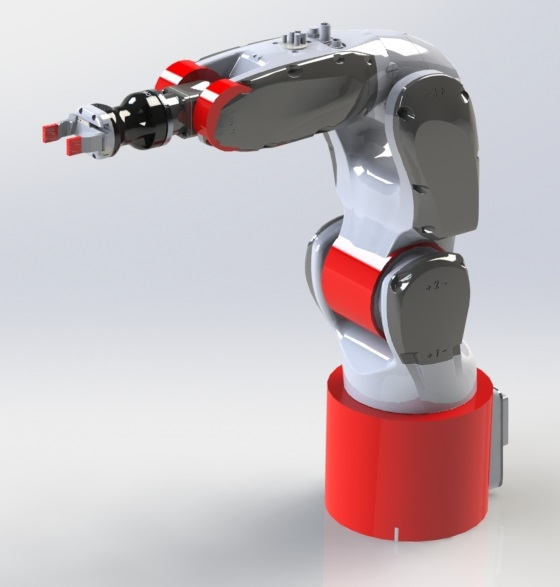
\includegraphics[width=0.35\textwidth]{Figures/CollShapes.JPG}
\caption{Collision Shapes (in Red)}
\end{figure}

Following this approach it is possible to reduce the computational time and the memory required by the training process, since contact detection and contact force evaluation becomes computationally lighter and triangular meshes are not even loaded in RAM since they are no longer required.

\subsubsection{Arm Contact}
Consider that because of body shapes, constraints and maximum allowed joints rotation only certain portion of the robotic arm can collide; moreover we are not interested in evaluating the exact contact but only in detecting the collision to penalize the reward in order to instruct the policy to avoid self collision.
\subsubsection{Fingers Contact}
The contact between the fingers and the box, on the contrary, has to be modelled precisely, but in many cases, such as this one, fingertips can also be modeled with contact primitive, as shown in figure 2 (contact shapes are in red).

\begin{figure} \label{FingerCS}
\centering
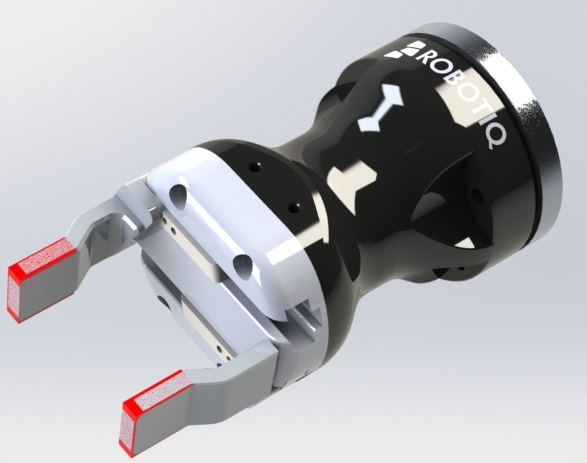
\includegraphics[width=0.3\textwidth]{Figures/Finger_CS.JPG}
\caption{Fingers Collision Shapes Closeup}
\end{figure}


\section{Robotic Environment}
\begin{figure} \label{ComauR3}
\centering
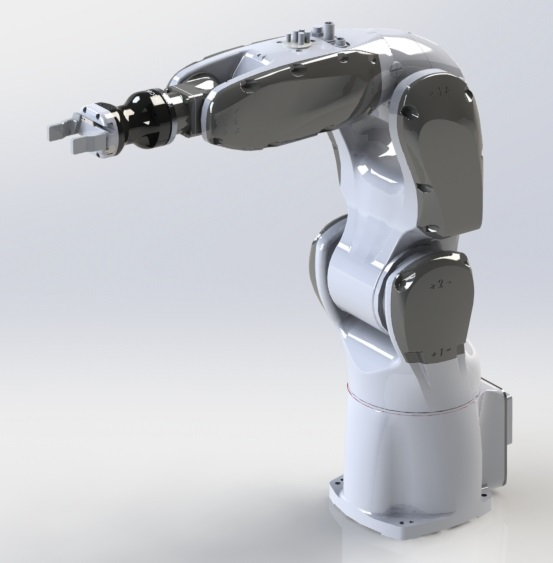
\includegraphics[width=0.35\textwidth]{Figures/RobotRender.JPG}
\caption{The Comau- Racer-3 6DOF Robot}
\end{figure}
The virtual environment is composed of a 6DOF robotic arm fixed on a planar surface, on which a small cubic box is rested. A 2 finger robotic hand is coupled to the robotic arm but the finger cannot move since in this example we have not introduced pick and place yet. The agent must learn to control the robot such that its fingertips reach and keep the position of the box center. 

The agent must also avoid:
\begin{itemize}
    \item Collisions between robotic arm parts.
    \item Collisions between the robot fingers and the table.
    \item Energy wasting policies
    \item Stuck joints
\end{itemize}

\subsection{States and Actions}
The state $s \in \mathbb{R}^{18}$ is composed of the potions and velocities of the robot joints ($\in \mathbb{R}^{12}$), the target position and the end effector position (both $\in \mathbb{R}^{3}$). 

The actions are the 6 motor torques. 
\subsection{Reward Shaping}

The reward is shaped as follows:

\begin{equation} \label{eq:Reward}
    r = \frac{r_d}{d+\epsilon} + S_c + F_c + c_e \left\Vert  T \omega \right\Vert + c_j S_j
\end{equation}
Where:
\begin{itemize}
    \item $r$ and $c$ are reward and cost constant coefficients referred to distance, energy and stuck joints (\textit{d, e, j} subscripts).
    \item $d$ is the distance between the fingers and the objective, while $\epsilon=0.0001$ avoids division by 0.
    \item $F_c$ is the finger contact penalty, equal to:
    
    $-\left(\left\Vert F_{f1}\right\Vert + \left\Vert F_{f2}\right\Vert \right)$ 
    
    where  $F_{f1}$ and $F_{f2}$ are the contact forces on the 2 fingers.
    \item $A_c$ is the arm collision penalty, equals to -1000 whenever any part of the robot (except fingers) collide.
    \item $T$ and $\omega$ are the vectors  motor torques and speed, whose dot product is the vector of motor powers.
    \item $S_j$ is the number of stuck joints (a joint is stuck when its rotation is equal to its maximum rotation).
\end{itemize}
Moreover, if $A_c<0$ (which means that a body of the robotic arm is colliding), the episode is reset so that the agent cannot collect any reward afterwards.

\section{DRL Algorithm}
\subsection{Proximal Policy Optimization}
Policy Gradient Methods are, in general, particularly suitable for tasks involving continuous states and actions (such as robotic tasks), and Proximal Policy Optimization has shown to perform well in robotic control applications \cite{openai2018HandManipulation}. 


The objective function for the parameter optimization in the implementation of the penalized version of the PPO algorithm \cite{Heess2017} is:
\begin{align*}
       \sum_{t=0}^\infty\gamma^t\frac{\pi_{\theta}(a_t|s_t)}{\pi_{\theta_{old}}(a_t|s_t)}
       A^{\pi, \gamma}(s_t,a_t)  -\beta_kD_{KL}(\theta_{old}||\theta) \\
        -\eta \max(0, D_{KL}(\theta_{old}||\theta) - 2KL_{targ})^2
\end{align*}
Where 
\begin{itemize}
    \item $\theta$ is the set of NN parameters (\emph{old} is their value at the beginning of the epoch). 
    \item $D_{KL}(\theta_{old}||\theta)$ is the Kullback-Leibler divergence between the policy at the beginning of the optimization epoch and the last policy.
    \item $KL_{targ}$ is the target value of the Kullback-Leibler divergence
    \item $\beta_k$ and $\eta$ are penalty coefficient used to penalize large policy updates.
    \item $A^\pi(s_t,a_t)$ is the Advantage Function
    \item $\gamma$ is the discount factor, used to reduce the relevance of future rewards.
\end{itemize}
We recall the definitions of discounted Value Function $V^{\pi, \gamma}(s_t)$: the expected sum of discounted rewards in the state $s_t$ at time $t$ following the policy $\pi$. 
\begin{equation}\label{eq_ValueFunc}
    V^{\pi, \gamma}(s_t) := E_{\underset{a_{t:\infty}}{s_{t+1:\infty}}}
    \left[\sum_{l=0}^\infty \gamma^l r_{t+l}\right]
\end{equation}

And discounted Advantage function  $A^{\pi, \gamma}(a_t,s_t)$ which is the advantage (in terms of reward) at timestep $t$ in state $s_t$, of taking the action $a_t$ and then following the policy, compared to following the policy.
\begin{equation} \label{eq:AdvFunc}
    A^{\pi, \gamma} = E_{s^{t+1}}\left[r_t+\gamma V^{\pi,\gamma}(s_{t+1})- V^{\pi,\gamma}(s_t)\right]
\end{equation}

To estimate the Advantage Function we trained a NN to estimate $V^{\pi, \gamma}(s_t)$, and then $A^{\pi, \gamma}(a_t,s_t)$ can be evaluated as suggested by Schulman et al. \cite{Schulman15GAE}.

The Kullback-Leibler divergence penalties prevents large parameters update avoiding the divergence of the policy; the KL divergence is indeed a measure of the difference between the two distributions.

PPO is an Actor-Critic algorithm: the Actor is NN actually prescribing the action  to the agent (the Policy), while the Critic in another Neural Network whose purpose is estimating the Critic performance, in our case by estimating the Value Function.


\subsection{NN Architecture}
We used fully connected NN with tanh activation function for both (Actor and Critic).
The policy NN has 18 inputs (the number of states), 6 outputs (the number of actions) and 3 hidden layers of 180, 104 and 60 neurons respectively.

The Critic NN has of course 18 inputs as well, and 1 output (the estimated value function). The 3 hidden layers have 180, 42 and 10 neurons respectively.
\section{Results}
\subsection{Comau Racer3}

\begin{figure}[ht] \label{Objective}
\centering
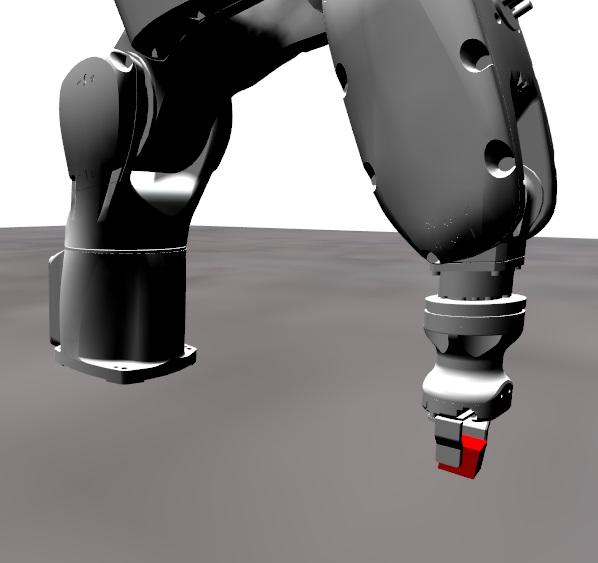
\includegraphics[width=0.3\textwidth]{Figures/objective.jpg}
\caption{Comau R3 Reaching Target Position }
\end{figure}

After 20000 training episodes the NN is able to control the robotic arm motor torques in order to reach a random position within a working area. The final position can be seen in Figure  4, and the learning progression is reported in Figure 5.
In addition, the control Policy learned to minimize energy consumption and contacts on the gripper fingers and above all, contacts between the robotic arm parts are always avoided. 
Using the simulation render to observe the Policy behaviour it can be noted that visualization shapes never overlap, demonstrating that using a limited number of contact primitives is indeed sufficient to avoid collisions between the real shapes. As can be seen in Figure 6 after the first half of the training, as soon as the Policy begins to undertake the wanted behavior, the episodes always last 3 seconds: since the agent dies if there is a collision between robotic arm parts, this means that they never happen after 10000 episodes of training.

It can also be noted that the policy learns to avoid unwanted collision first, then it learns to bring the end effector in the right position. 

\begin{figure}[ht] \label{R3RewPlot}
\centering
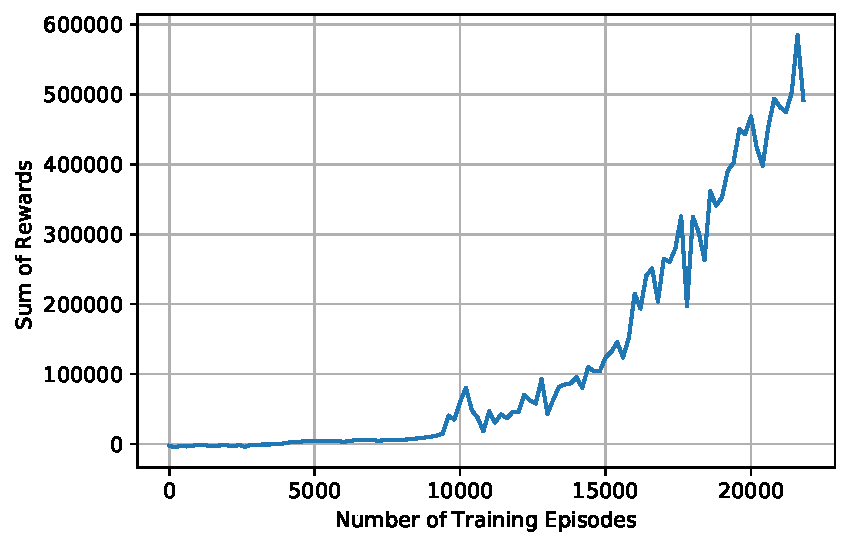
\includegraphics[width=0.3\textwidth]{Plots/R3Rew.pdf}
\caption{Comau R3 Sum Of Collected \newline Rewards (10 Batches Mean)}
\end{figure}

\begin{figure}[ht] \label{R3TimePlot}
\centering
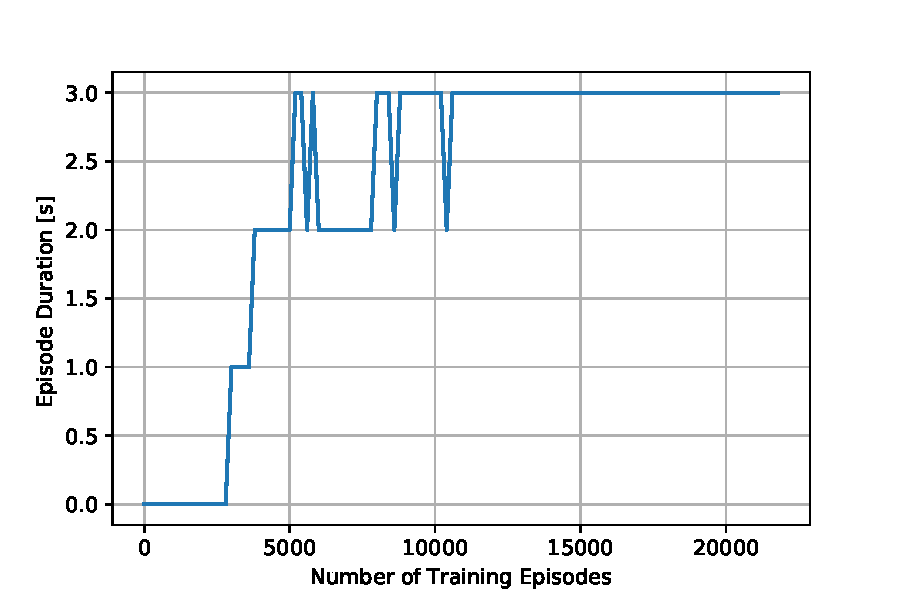
\includegraphics[width=0.3\textwidth]{Plots/R3Time.pdf}
\caption{Comau R3 Episode Duration \newline (10 Batches Mean)}
\end{figure}

\subsubsection{Transferring the Policy}
Training an agent on a simple task and then transfer the learning in a more complex environment is a well studied strategy and has also been applied in deep reinforcement learning for continuous control problems \cite{Berseth18}.
%
%\paragraph{Constant to Random Position}

Training the agent to reach an object whose position is fixed and then training the same policy to reach a random position within a working area proved to be a poor strategy, as shown in the plot in Figure 7. The policy performance is bad and the benefit in term of training time is negligible  compared to training with a random object position from scratch as previously shown.

The limited training speedup discouraged us from considering more advanced transfer learning techniques.

\begin{figure}[ht] \label{R3ConstToRand}
\centering
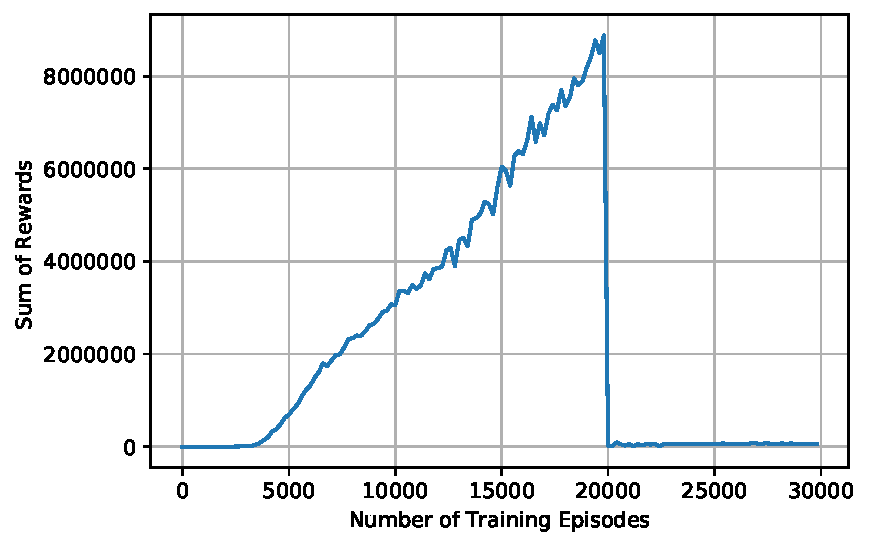
\includegraphics[width=0.3\textwidth]{Plots/R3_C_to_Rand_Rew.pdf}
\caption{Switching from fixed to random position after 20000 episodes. Sum of rewards
(10 B Mean)}
\end{figure}


%\paragraph{Fixed to Moving Objective Box}

\subsection{ABB IRB 120}
Finally, we used the same procedure to train a different robotic arm. We choose the ABB IRB 120 because it is similar in terms of working area and payload to the Comau Racer3, thus they can be both used in the same applications. 

Here we fully exploited the versatility of our simulation platform, since except for collision shapes in the CAD and maximum rotations, velocities and torques in the code, we did not have to introduce modifications.

In Figure 8 is reported the learning progression while Figure 9 is a render frame of the simulation of the trained Policy.

\begin{figure}[ht] \label{ABB_Rew}
\centering
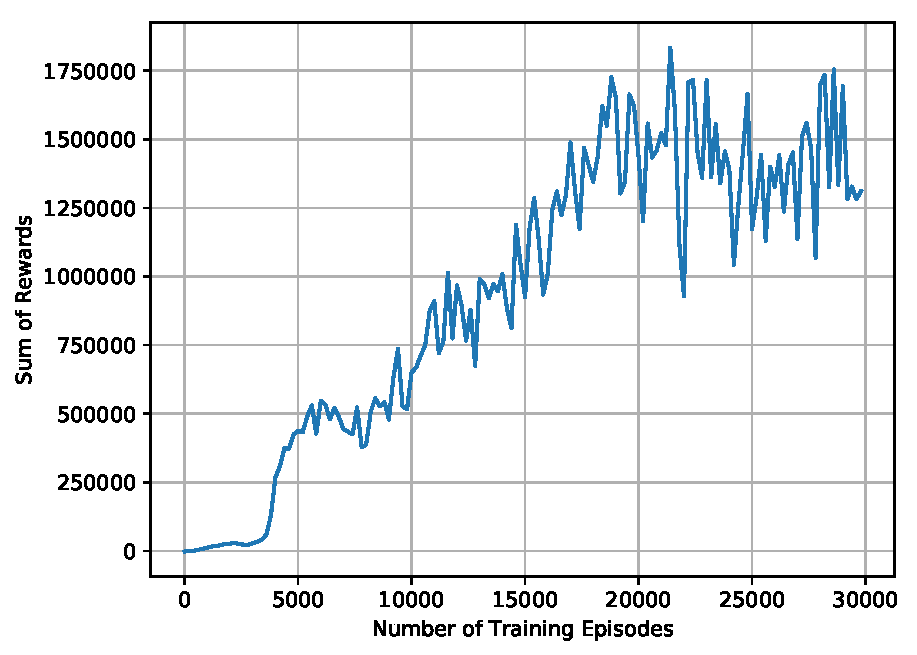
\includegraphics[width=0.3\textwidth]{Plots/ABB_Rew.pdf}
\caption{ABB IRB 120 Sum Of Collected \newline Rewards (10 Batches Mean)}
\end{figure}

\begin{figure}[ht] \label{ABB}
\centering
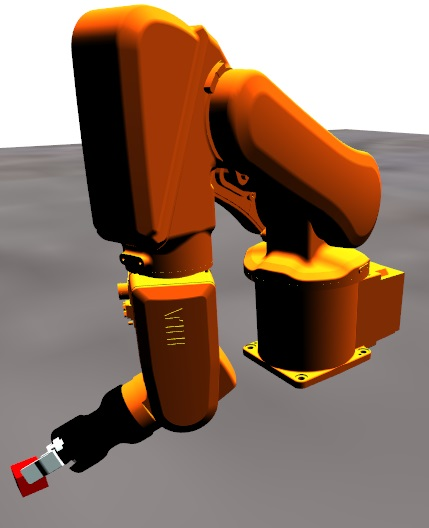
\includegraphics[width=0.3\textwidth]{Figures/ABB.jpg}
\caption{ABB IRB 120 Reaching Target Position}
\end{figure}

%\subsection{Object Following}
\section{Conclusions}
After the results previously shown, we can state that:
\begin{itemize}
    \item Physical model for NN training can be built in CAD software This approach is user-friendly and above all versatile: once the simulation environment is set up minor changes in the model (such as dimensions, positions of mass properties) can be automatically passed to the simulation.
    \item Since all 6DOF robotic arms share the same structure (7 bodies connected by 6 revolute joints), changing the robotic arm model requires minimal modifications.
    Indeed, passing from the Comau Racer3 to the ABB IRB 120 required to modify only the hard coded specifications of the robotic arm. 
    
    The possibility of applying the same algorithm to different robotic arms will be especially welcome when industrial applications of NN-controlled robots will start to spread.
    \item A small number of contact primitives can be effectively used to train the Policy to avoid collisions.
    
\end{itemize}

Furthermore, we plan to use this approach together with Convolutional Neural Networks fed with  images from simulation render to train visuomotor policies.

%\begin{figure*}
%\centering
%\includegraphics{flies}
%\caption{A sample black and white graphic
%that needs to span two columns of text.}
%\end{figure*}

\section{Acknowledgments}

This research benefits from the HPC (High Performance Computing) facility of the University of Parma, Italy.


\printbibliography


\end{document}
